%\setchapterimage{Fond_CIN.png}
\setchapterpreamble[u]{\margintoc}

\chapter{Génie électrique en tension alternative}


%\marginnote[4cm]{
%\UPSTIcompetence[2]{B2-10}
%}

%\marginnote[6cm]{\textbf{Emilien Durif}, \textit{Approche énergétique}, Lycée La Martinière Monplaisir, Lyon.}

\section{Signaux périodiques}

\subsection{Caractéristique des signaux périodiques}

\begin{marginfigure}
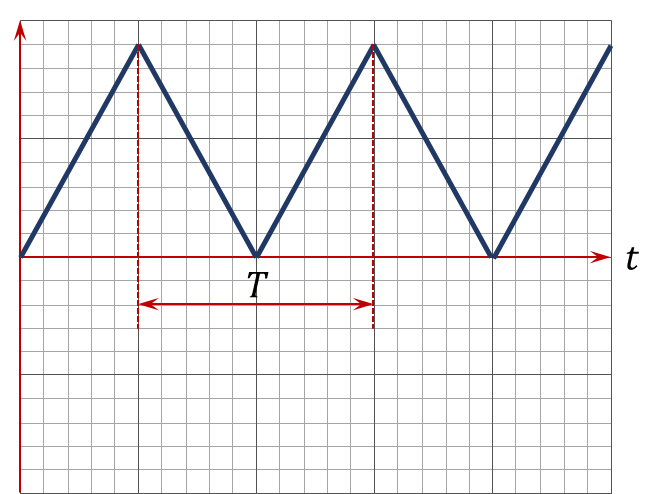
\includegraphics[width=\linewidth]{fig_01}
\caption{Signal périodique \label{fig:ge:cours:01}}
\end{marginfigure}

\begin{defi}[Signal périodique]
Un signal $s(t)$ est dit périodique de période $T$ si $\forall t$, $s(t)=s(t+T)$.
\end{defi}

\begin{defi}[Caractéristiques]
On peut définir : 
\begin{itemize}
\item la fréquence du signal, en Hertz \si{Hz}, $f=\dfrac{1}{T}$;
\item la pulsation, pour un régime sinusoïdal, en \si{rad.s^{-1}} :  $\omega = 2\pi f$;
\item la valeur maximale (ou de crête). 
\end{itemize}
\end{defi}

\subsection{Valeur moyenne}
\begin{marginfigure}
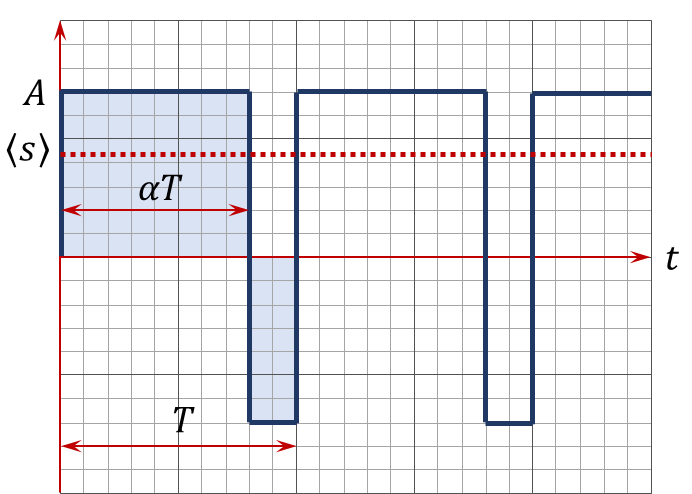
\includegraphics[width=\linewidth]{fig_02}
\caption{Valeur moyenne\label{fig:ge:cours:02}}
\end{marginfigure}


\begin{marginfigure}
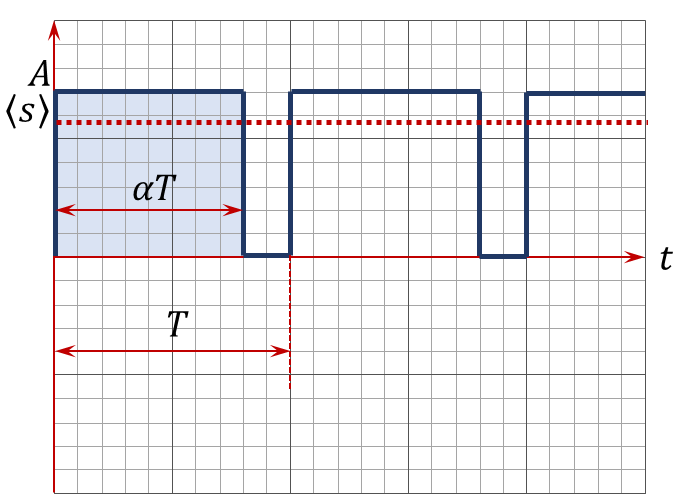
\includegraphics[width=\linewidth]{fig_03}
\caption{Valeur moyenne\label{fig:ge:cours:03}}
\end{marginfigure}

\begin{defi}[Valeur moyenne]
Valeur de la grandeur continue qui créerait la même aire qu'un signal périodique sur une période $T$.
On a alors : 
$$\langle s \rangle = \dfrac{1}{T} \int\limits_{t_0}^{t_0+T} s(t)\; \dd t.$$
\end{defi}

\begin{prop}
Si $s(t) = s_1(t)+s_2(t)$ alors  $\langle s \rangle = \langle s_1 \rangle+\langle s_2 \rangle$.
\end{prop}

La valeur moyenne est celle mesurée par un multimètre en position \textbf{DC} ou \textbf{=}.
